%=============================================================================
% APPENDIX D: EXPERIMENTAL PROTOCOLS
% DFD Unified Review
%=============================================================================

\section{Experimental Protocols}\label{app:protocols-D}

This appendix specifies technical requirements for the key experiments 
that can test \DFD predictions. The goal is to enable independent 
replication and provide guidance for experimentalists.

%-----------------------------------------------------------------------------
% D.1 CLOCK COMPARISON PROCEDURE
%-----------------------------------------------------------------------------
\subsection{Clock Comparison Procedure}\label{app:clock_protocol}

\subsubsection{Measurement Overview}

The clock anomaly test searches for species-dependent gravitational 
coupling by comparing frequency ratios of different clock types as 
Earth's distance to the Sun varies through the year.

\paragraph{Observable:}
\begin{equation}
y_{AB}(t) = \frac{\nu_A(t) - \nu_B(t)}{\nu_A} - \langle y_{AB}\rangle,
\end{equation}
where $A$ and $B$ are clock types with different $\alpha$-sensitivities.

\paragraph{Expected Signal:}
\begin{equation}
y_{AB}(t) = (K_A - K_B)\frac{\Delta\Phi_\odot(t)}{c^2},
\end{equation}
where $\Delta\Phi_\odot(t)$ varies by $\pm 3.3 \times 10^{-10}$ annually.

\subsubsection{Technical Requirements}

\begin{table}[h!]
\centering
\caption{Clock comparison technical specifications.}
\label{tab:clock_specs}
\resizebox{\columnwidth}{!}{%
\begin{tabular}{lll}
\toprule
\textbf{Parameter} & \textbf{Requirement} & \textbf{Current State} \\
\midrule
Fractional stability & $\sigma_y < 10^{-16}$ @ 1 day & Achieved (Sr, Yb$^+$) \\
Systematic uncertainty & $< 10^{-17}$ & Achieved (best optical) \\
Measurement duration & $> 1$ year (ideally 2--3) & Standard campaigns \\
Sampling rate & Daily or better & Standard \\
Clock pair $\Delta S^\alpha$ & $> 2$ (maximize signal) & Cs--Sr: $\Delta S = 2.77$ \\
Environmental control & mK temperature stability & Standard \\
Vibration isolation & $< 10^{-9}g$ @ 1 Hz & Standard \\
\bottomrule
\end{tabular}
}% end resizebox
\end{table}

\subsubsection{Recommended Clock Pairs}

\begin{enumerate}
\item \textbf{Primary:} Cs hyperfine -- Sr optical
   \begin{itemize}
   \item $\Delta S^\alpha = 2.83 - 0.06 = 2.77$
   \item Expected signal: $\Delta y \sim 2.4 \times 10^{-5} \times 6 \times 10^{-10} \sim 1.4 \times 10^{-14}$ (annual)
   \end{itemize}

\item \textbf{Enhanced:} Yb$^+$ E3 -- Al$^+$
   \begin{itemize}
   \item $\Delta S^\alpha = -5.95 - 0.008 = -5.96$
   \item Larger signal amplitude
   \item Both optical (reduced systematics)
   \end{itemize}

\item \textbf{Null control:} Sr -- Yb ($^1S_0$--$^3P_0$)
   \begin{itemize}
   \item $\Delta S^\alpha = 0.06 - 0.31 = -0.25$
   \item Small $\Delta S$ serves as null check
   \end{itemize}
\end{enumerate}

\subsubsection{Data Analysis}

\paragraph{Step 1: Time Series Construction.}
Record frequency ratio $\nu_A/\nu_B$ vs.\ modified Julian date (MJD).

\paragraph{Step 2: Template Fitting.}
Fit to:
\begin{equation}
y(t) = A_0 + A_1 t + A_\Phi \cdot \frac{\Phi_\odot(t)}{c^2} + \text{systematics},
\end{equation}
where $\Phi_\odot(t) = -GM_\odot/r_\oplus(t)$.

\paragraph{Step 3: Extract $\Delta K$.}
\begin{equation}
K_A - K_B = \frac{A_\Phi}{|\Delta\Phi_\odot|_{\rm max}} \approx \frac{A_\Phi}{3.3 \times 10^{-10}}.
\end{equation}

\paragraph{Step 4: Compare to Prediction.}
\begin{equation}
(K_A - K_B)_{\DFD} = \kalpha \cdot \Delta S^\alpha = \frac{\alpha^2}{2\pi}\Delta S^\alpha.
\end{equation}

\subsubsection{Systematic Error Budget}

\begin{table}[h!]
\centering
\caption{Systematic error budget for clock comparison.}
\label{tab:clock_systematics}
\begin{tabular}{lll}
\toprule
\textbf{Effect} & \textbf{Magnitude} & \textbf{Mitigation} \\
\midrule
Blackbody radiation & $\sim 10^{-16}$ & Temperature control \\
Zeeman shifts & $\sim 10^{-17}$ & Magnetic shielding \\
Gravitational redshift & $\sim 10^{-16}$ h$^{-1}$ & Height measurement \\
Reference cavity drift & $\sim 10^{-17}$/day & Co-located comparison \\
Annual temperature cycle & Variable & Monitor and correct \\
Tidal effects & $\sim 10^{-17}$ & Model and subtract \\
\bottomrule
\end{tabular}
\end{table}

\subsubsection{Windowed vs.\ Global Analysis Strategies}

Two complementary approaches exist for extracting annual gravitational signals:

\paragraph{Global year-long fit.}
Fit the full multi-year dataset with a flexible drift model (polynomials, splines) plus the gravitational template $\Phi_\odot(t)$. Advantages: robust statistics, clear identification of sinusoidal annual signal. Risk: flexible drift models can partially absorb the gravitational template, especially if the signal is weak.

\paragraph{Perihelion-windowed analysis.}
Analyze a focused window (30--60 days) around perihelion where $d\Phi_\odot/dt$ is maximal. Use only linear drift within the window. Advantages: sensitive to the \textit{shape} of the potential variation; less prone to drift absorption. Risk: shorter baseline increases degeneracy with instrumental drift.

\paragraph{Recommended protocol.}
\begin{enumerate}
\item Perform both analyses and report both results.
\item Quantify the covariance between drift and potential coefficients in each case.
\item A robust signal should appear in both approaches; discrepancy indicates systematic concerns.
\item Preserve and publish raw ratios to enable independent reanalysis.
\end{enumerate}

The windowed approach is particularly valuable when exploring marginal hints, as aggressive global detrending can project out exactly the annual structure one seeks to test.

%-----------------------------------------------------------------------------
% D.2 CAVITY-ATOM LPI TEST
%-----------------------------------------------------------------------------
\subsection{Cavity-Atom Setup Requirements}\label{app:cavity_atom}

\subsubsection{Experiment Concept}

Compare an optical cavity (photon sector) to an atomic clock (matter sector) 
while varying gravitational potential. \DFD predicts different responses, 
with \GR predicting $\xi_{\rm LPI}^{\GR}=0$ and corrected \DFD predicting only a screened residual $\xi_{\rm LPI}^{\rm res}$ once the constitutive-chain cancellation is imposed.

\subsubsection{Key Configuration}

\begin{figure}[h!]
\centering
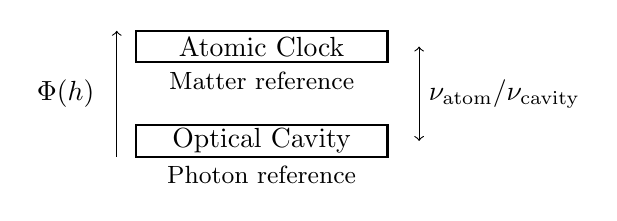
\begin{tikzpicture}[scale=0.8]
% Cavity
\draw[thick] (0,0) rectangle (4,0.5);
\node at (2,0.25) {Optical Cavity};
\node[below] at (2,0) {\small Photon reference};

% Atom
\draw[thick] (0,1.5) rectangle (4,2);
\node at (2,1.75) {Atomic Clock};
\node[below] at (2,1.5) {\small Matter reference};

% Comparison
\draw[<->] (4.5,0.25) -- (4.5,1.75);
\node[right] at (4.5,1) {$\nu_{\rm atom}/\nu_{\rm cavity}$};

% Potential
\node[left] at (-0.5,1) {$\Phi(h)$};
\draw[->] (-0.3,0) -- (-0.3,2);
\end{tikzpicture}
\caption{Schematic of cavity-atom comparison.}
\end{figure}

\subsubsection{Technical Specifications}

\begin{table}[h!]
\centering
\caption{Cavity-atom test specifications.}
\label{tab:cavity_atom_specs}
\resizebox{\columnwidth}{!}{%
\begin{tabular}{lll}
\toprule
\textbf{Component} & \textbf{Requirement} & \textbf{Notes} \\
\midrule
Cavity finesse & $> 10^5$ & ULE or Si spacer \\
Cavity stability & $< 10^{-16}$ @ 1 s & Temperature stabilized \\
Atom clock & Sr or Yb optical & $< 10^{-18}$ systematic \\
$\Delta\Phi/c^2$ variation & $> 10^{-12}$ & Height change or orbital \\
Measurement duration & $> 10^4$ s per height & Statistics \\
Height separation & $> 10$ m (terrestrial) & Tower or elevator \\
\bottomrule
\end{tabular}
}% end resizebox
\end{table}

\subsubsection{Height Comparison Method}

\paragraph{Configuration A: Tower Experiment}
\begin{itemize}
\item Cavity at ground level
\item Atomic ensemble transported to height $h$
\item Compare via fiber link
\item $\Delta\Phi/c^2 = gh/c^2 \approx 10^{-15}$ per 100 m
\end{itemize}

\paragraph{Configuration B: Space Mission}
\begin{itemize}
\item Cavity and atoms on same platform
\item Vary orbital altitude
\item $\Delta\Phi/c^2 \sim 10^{-10}$ (LEO to higher orbit)
\item Enhanced signal but complex mission
\end{itemize}

\subsubsection{Observable}

\begin{equation}
\frac{d}{d\Phi}\left(\frac{\nu_{\rm atom}}{\nu_{\rm cavity}}\right) = \frac{\xi_{\rm LPI}}{c^2},
\end{equation}
where $\xi_{\rm LPI}^{\GR}=0$ and the corrected \DFD expectation is a small screened residual rather than an order-unity slope.

\subsubsection{Discrimination Significance}

With current technology:
\begin{itemize}
\item 100 m height: $\Delta\Phi/c^2 \approx 10^{-15}$
\item Clock comparison at $10^{-18}$: useful only for a residual-level cavity--atom search
\item \textbf{Discrimination now requires pushing into the screened-residual regime rather than separating $\xi_{\rm LPI}=0$ from an order-unity value}
\end{itemize}

%-----------------------------------------------------------------------------
% D.3 MATTER-WAVE INTERFEROMETER
%-----------------------------------------------------------------------------
\subsection{Matter-Wave Interferometer Specifications}\label{app:matter_wave_protocol}

\subsubsection{Target Signal}

The \DFD-specific phase shift is:
\begin{equation}
\Delta\phi_{\DFD} = \frac{\hbar k_{\rm eff}^2}{m}\frac{g}{c^2}T^3 \cdot K_{\rm atom}.
\end{equation}

With $K_{\rm atom} \sim 10^{-5}$ and accessible parameters, sensitivity 
requires $T \gtrsim 1$ s and phase resolution $< 10^{-9}$ rad.

\subsubsection{Interferometer Requirements}

\begin{table}[h!]
\centering
\caption{Matter-wave interferometer specifications for \DFD test.}
\label{tab:mw_specs}
\resizebox{\columnwidth}{!}{%
\begin{tabular}{llll}
\toprule
\textbf{Parameter} & \textbf{Minimum} & \textbf{Target} & \textbf{Notes} \\
\midrule
Free-fall time $T$ & 0.5 s & 2 s & Limits signal \\
$k_{\rm eff}$ & $10^7$ m$^{-1}$ & $2 \times 10^7$ m$^{-1}$ & Two-photon Raman \\
Phase resolution & $10^{-8}$ rad & $10^{-10}$ rad & Shot noise limit \\
Atom number & $10^5$ & $10^7$ & Statistics \\
Systematic control & $10^{-9}$ rad & $10^{-10}$ rad & Gravity gradients \\
Species & $^{87}$Rb & $^{87}$Rb, $^{85}$Rb & Comparison \\
\bottomrule
\end{tabular}
}% end resizebox
\end{table}

\subsubsection{Dual-Species Configuration}

To extract the species-dependent $K_{\rm atom}$:
\begin{enumerate}
\item Run identical interferometer with $^{87}$Rb and $^{85}$Rb
\item Both have same $m_{\rm Rb}$ to $< 2\%$
\item Different $S^\alpha$ values
\item Differential measurement cancels common-mode systematics
\end{enumerate}

\subsubsection{$T^3$ Signature}

The \DFD signal scales as $T^3$, while:
\begin{itemize}
\item Standard gravitational phase $\propto T^2$
\item Gravity gradient phase $\propto T^4$
\item Rotation phase $\propto T^2$
\end{itemize}

This distinct scaling provides an orthogonal discriminator.

\subsubsection{Systematic Control}

\begin{table}[h!]
\centering
\caption{Matter-wave systematic errors.}
\label{tab:mw_systematics}
\begin{tabular}{lll}
\toprule
\textbf{Effect} & \textbf{Scaling} & \textbf{Mitigation} \\
\midrule
Gravity gradient & $T^4$ & Gradient compensation \\
Coriolis force & $T^2$ & Rotation compensation \\
Laser wavefront & $T^2$ & High-quality optics \\
AC Stark shift & Independent & Laser intensity control \\
Magnetic fields & $T^2$ & Magnetic shielding \\
Two-photon light shift & $T^2$ & Symmetric pulse \\
\bottomrule
\end{tabular}
\end{table}

%-----------------------------------------------------------------------------
% D.4 ROTATION CURVE ANALYSIS
%-----------------------------------------------------------------------------
\subsection{Galaxy Rotation Curve Analysis}\label{app:rotation_protocol}

\subsubsection{Data Requirements}

\begin{itemize}
\item \textbf{Rotation curve:} HI 21cm and/or H$\alpha$ emission
\item \textbf{Resolution:} Beam size $< 1$ kpc at galaxy distance
\item \textbf{Velocity precision:} $< 5$ km/s per point
\item \textbf{Radial extent:} Out to $\gtrsim 3$ disk scale lengths
\item \textbf{Inclination:} $30^\circ < i < 80^\circ$ (avoid edge-on/face-on)
\end{itemize}

\subsubsection{Baryonic Mass Model}

\begin{enumerate}
\item \textbf{Stellar mass:} From 3.6 $\mu$m photometry
   \begin{equation}
   \Sigma_\star(r) = \Upsilon_\star \cdot I_{3.6}(r)
   \end{equation}
   with $\Upsilon_\star \approx 0.5$ $M_\odot/L_\odot$ (disk)

\item \textbf{Gas mass:} From HI 21cm + correction for He
   \begin{equation}
   \Sigma_{\rm gas} = 1.33 \cdot \Sigma_{\rm HI}
   \end{equation}

\item \textbf{Total:}
   \begin{equation}
   V_{\rm bar}^2(r) = V_\star^2(r) + V_{\rm gas}^2(r)
   \end{equation}
\end{enumerate}

\subsubsection{DFD Fitting Procedure}

\paragraph{Step 1:} Compute $g_{\rm bar}(r) = V_{\rm bar}^2(r)/r$

\paragraph{Step 2:} Apply interpolating function:
\begin{equation}
g_{\rm obs}(r) = g_{\rm bar}(r) \cdot \nu\left(\frac{g_{\rm bar}(r)}{a_0}\right)
\end{equation}

\paragraph{Step 3:} Convert to velocity:
\begin{equation}
V_{\DFD}(r) = \sqrt{r \cdot g_{\rm obs}(r)}
\end{equation}

\paragraph{Step 4:} Minimize $\chi^2$:
\begin{equation}
\chi^2 = \sum_i \frac{[V_{\rm obs}(r_i) - V_{\DFD}(r_i)]^2}{\sigma_i^2}
\end{equation}
with free parameters: $a_0$ (or fixed), $\Upsilon_\star$, distance.

\subsubsection{Quality Metrics}

\begin{itemize}
\item $\chi^2$/dof $< 2$ (good fit)
\item Residuals randomly distributed (no systematic trends)
\item $\Upsilon_\star$ consistent with stellar population models
\item $a_0$ consistent across galaxy sample
\end{itemize}

%-----------------------------------------------------------------------------
% D.5 RECIPROCITY-BROKEN FIBER LOOP
%-----------------------------------------------------------------------------
\subsection{Reciprocity-Broken Fiber Loop Protocol}\label{app:fiber_loop}

A non-reciprocal phase accumulation in a closed fiber path provides a direct, 
clock-independent test of the \DFD refractive potential.

\subsubsection{Physical Principle}

In \DFD, light propagating through a medium with refractive index $n = e^\psi$ 
accumulates optical phase. For a \emph{closed} path $C$, the non-reciprocal 
residue from $\psi$ gradients is:
\begin{equation}\label{eq:phi-NR}
\boxed{\Delta\phi_{\rm NR} = \frac{\omega}{c}\oint_C \psi\,ds}
\end{equation}
This achromatic phase offset directly probes the line integral of $\psi$ 
around the closed loop.

\subsubsection{Configuration: Vertical Loop}

Consider two horizontal fiber arms at heights $z_T$ (top) and $z_B$ (bottom) 
with lengths $L_T$ and $L_B$, connected by short vertical risers. Near Earth's 
surface, $\psi \simeq -2gz/c^2$, giving:
\begin{equation}\label{eq:fiber-phase}
\Delta\phi_{\rm NR} \simeq -\frac{2\omega g}{c^3}(z_T L_T - z_B L_B).
\end{equation}

For a symmetric rectangular loop with $L_T = L_B = L$ and vertical separation 
$\Delta z = z_T - z_B$:
\begin{equation}\label{eq:fiber-rect}
\Delta\phi_{\rm NR} \simeq -\frac{2\omega g L \Delta z}{c^3}.
\end{equation}

\paragraph{Numerical example.}
For $L = 100$~m, $\Delta z = 10$~m, $\omega/2\pi = 193$~THz (1550~nm telecom):
$\Delta\phi_{\rm NR} \approx 9 \times 10^{-6}$~rad $\approx 5~\mu$rad.
This is detectable with heterodyne interferometry at $\sim\mu$rad sensitivity.

\subsubsection{Dual-Wavelength Dispersion Check}

Material dispersion produces wavelength-dependent phase shifts that could 
mimic the signal. A dual-wavelength measurement provides a critical discriminator:
\begin{equation}\label{eq:dual-lambda}
\mathcal{D} \equiv \Delta\phi(\lambda_1) - \frac{\lambda_1}{\lambda_2}\Delta\phi(\lambda_2)
\end{equation}
vanishes for the achromatic DFD signal but is nonzero for dispersive contamination. 
Running at two wavelengths (e.g., 1550~nm and 780~nm) isolates the $\psi$-contribution.

\subsubsection{Systematic Error Budget}

\begin{table}[h!]
\centering
\caption{Fiber loop systematic error budget.}
\label{tab:fiber-systematics}
\scriptsize
\setlength{\tabcolsep}{2pt}
\begin{tabular}{lll}
\toprule
\textbf{Effect} & \textbf{Magnitude} & \textbf{Mitigation} \\
\midrule
Material dispersion & $\sim 10^{-4}$~rad/m & Dual-$\lambda$ check \\
Sagnac rotation & $\propto A \Omega$ & Common-path/gyro \\
Temperature drift & $\propto dn/dT$ & Stabilization ($\pm 1$~mK) \\
Fiber birefringence & $\sim 10^{-7}$~rad/m & PM fiber + pol.\ ctrl \\
\bottomrule
\end{tabular}
\end{table}

\subsubsection{Achievable Sensitivity}

With current technology:
\begin{itemize}
\item Phase resolution: $10^{-6}$~rad (heterodyne at 1~Hz bandwidth)
\item Signal (100~m $\times$ 10~m loop): $\sim 10^{-5}$~rad
\item \textbf{SNR $\gtrsim 10$ achievable with tabletop apparatus}
\end{itemize}

\paragraph{Falsification criterion.}
A null result at $\lesssim 10^{-6}$~rad with proper dispersion controls would 
constrain $|\psi - \psi_{\rm GR}| < 10^{-3}$ at laboratory scales.

%-----------------------------------------------------------------------------
% D.6 SUMMARY: DECISION MATRIX
%-----------------------------------------------------------------------------
\subsection{Decision Matrix: Which Experiment to Prioritize}\label{app:decision}

\begin{table}[h!]
\centering
\caption{Experimental decision matrix for \DFD tests.}
\label{tab:decision}
\resizebox{\columnwidth}{!}{%
\begin{tabular}{lccccc}
\toprule
\textbf{Experiment} & \textbf{Signal} & \textbf{Timescale} & \textbf{Cost} & \textbf{Discriminating} & \textbf{Priority} \\
\midrule
Clock anomaly & $10^{-15}$ & 1--2 yr & Low & Yes & High \\
Cavity-atom residual & screened residual & Long-term & Medium & Yes & Medium \\
Fiber loop & $\sim\mu$rad & 1 yr & Low & Yes & High \\
Matter-wave $T^3$ & $10^{-11}$ rad & 3--5 yr & Medium & Yes & Medium \\
Galaxy RAR & $< 0.15$ dex & Done & Low & No (confirms) & Complete \\
GW ppE & $\delta\hat\varphi = 0$ & Done & N/A & No (confirms) & Complete \\
\bottomrule
\end{tabular}
}% end resizebox
\end{table}

\paragraph{Recommendation:} The corrected near-term emphasis is on nuclear clocks and cross-species clock analyses.  Cavity--atom work remains valuable, but now as a long-horizon residual test rather than the first binary discriminator.  Matter-wave $T^3$ provides an orthogonal check.
